\documentclass[a4paper,11pt,fleqn]{article}%fleqn pour aligner les equations à gauche
\usepackage{../../Styles/Exercice}

\newcommand{\chnum}{Chapitre 18}
\newcommand{\chtitle}{Interférences et diffraction}
\newcommand{\dtype}{Exercices}

\begin{document}
\maketitle

\section{Périodicité d'une onde}
Une onde mécanique progressive sinusoïdale de fréquence $f$ = \SI{1,5}{\mega\hertz} et de phase à l'origine $\phi = \dfrac{\pi}{2}$ se propage avec une célérité $c$ = \SI{1500}{\meter\per\second}.
\begin{itemize}
    \item Déterminer la période $T$ ainsi que la longueur d'onde $\lambda$ de l'onde mécanique.
\end{itemize}
\textcolor{blue}{La période est accessible à travers la fréquence par la relation : $f=\dfrac{1}{T}$, soit $T = \dfrac{1}{f}$. Ici $T = \dfrac{1}{\num{1,5e6}}$ = \SI{6,7E-6}{\second}.\\
La longueur d'onde est accessible via la formule $c=\dfrac{\lambda}{T}$, soit $\lambda = \dfrac{c}{T}$, ici $\lambda = 1500 \times \num{6,7e-7}$ = \SI{1E-2}{\meter}}.\\

\section{Identification d'une onde sinusoïdale}
L'amplitude d'une onde mécanique est modélisée par la fonction suivante :
$$s(x,t)=2,0 \times \cos{\left( \dfrac{2\pi}{2,0 \times 10^{-3}} \times \left( t - \dfrac{x}{c}\right) + \dfrac{\pi}{3}\right)}$$
\begin{enumerate}
    \item À partir de l'expression ci-dessus, déterminer la valeur de la période $T$ et de la phase à l'origine $\phi$.\\
    \textcolor{blue}{Dans l'expression ci-dessous, par analogie avec la fonction d'une onde sinusoïdale de formule générale : $$s(x,t)=2,0 \times \cos{\left( \dfrac{2\pi}{T} \times \left( t - \dfrac{x}{c}\right) + \phi\right)}$$
    On peut déterminer que $T$ = \num{2,0e-3} \unit{\second} et que $\phi = \dfrac{\pi}{3}$ \unit{radian}}
    \item Déterminer la valeur de l'amplitude $s$ de l'onde à l'origine ($x$ et $t$ sont nuls).\\
    \textcolor{blue}{Lorsque $t$ et $x$ sont nuls, l'expression donne :
    $$s(0,0)=2,0 \times \cos{\left( \dfrac{2\pi}{2,0 \times 10^{-3}} \times \left( 0 - \dfrac{0}{c}\right) + \dfrac{\pi}{3}\right)} $$
    $$s(0,0)=2,0 \times \cos{\left(\dfrac{\pi}{3}\right)}$$
    $$\text{Soit : } s(0,0)=1 $$}
    \item À $x$ = \num{0} \unit{\meter}, représenter graphiquement l'évolution de l'amplitude de l'onde $s(x,t)$ sur une durée égale à $3T$ à la calculatrice.\\
    \textcolor{blue}{Pour $x$ = 0 m, la fonction devient : $s(x,t)=2,0 \times \cos{\left( \dfrac{2\pi}{\num{2,0e-3}} \times t + \dfrac{\pi}{3}\right)}$\\
    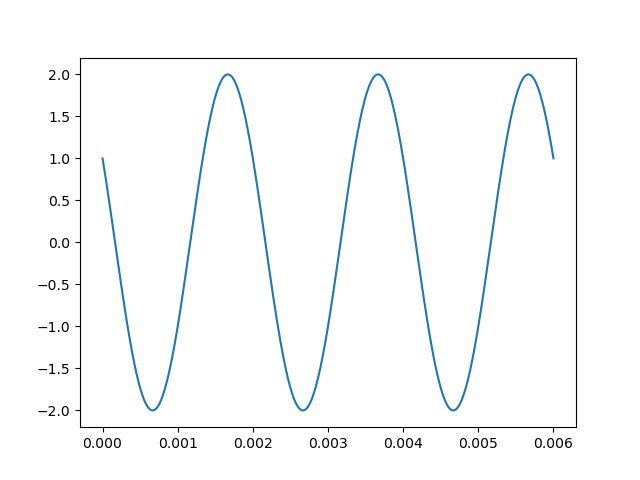
\includegraphics[scale = .5]{Ressources/TSPE_C9_Exercices_Fig6.png}}
    \item Sur le même graphique, représenter une onde identique mais dont le déphasage à l'origine est égal à zéro.\\
    \textcolor{blue}{Une onde avec une origine à 0 est une onde avec un déphasage $\phi$ = 0. On aura donc la fonction suivante : $s(x,t)=2,0 \times \cos{\left( \dfrac{2\pi}{\num{2,0e-3}} \times t \right)}$\\
    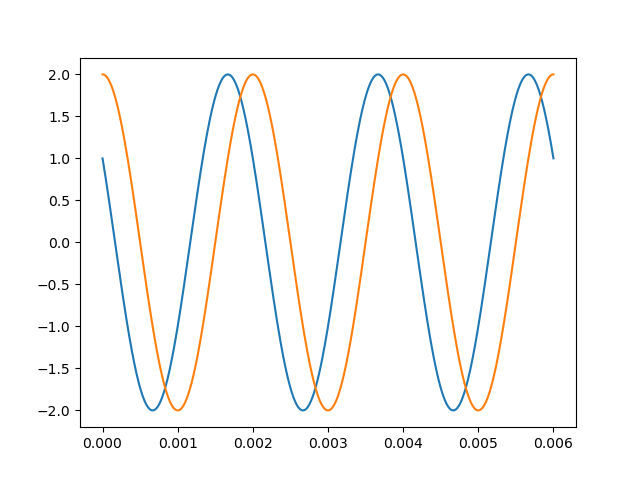
\includegraphics[scale =.5]{Ressources/TSPE_C9_Exercices_Fig7.png}}
\end{enumerate}

\section{Expérience d'Young}
Thomas Young élabore en 1801 un dispositif pour démontrer la nature ondulatoire de la lumière. Cette expérience est restée célèbre sous le nom d'expérience des trous d'Young. Vers 1818, le français Augustin Fresnel a l'idée de remplacer les trous par des fentes.
\begin{itemize}
    \item Parmi les trois photographies ci-dessous, identifier celles qui correspondent aux deux expériences décrites dans l'énoncé. Justifier.
\end{itemize}
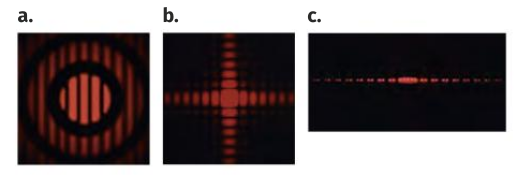
\includegraphics[scale =1]{Ressources/TSPE_C9_Exercices_Fig1.png}\\
\textcolor{blue}{La figure a. propose des taches de diffraction circulaires dans lesquelles on peut observer des figures d'interférence. La forme de diffraction suggère que l'obstacle a une forme circulaire et la présence d'interférences montre la présence de deux sources lumineuses cohérentes : Il s'agit de l'expérience des trous d'Young.\\
La figure b. présente des taches de diffraction verticales et horizontales, indiquant la présence d'un objet en forme de croix. Il n'y a pas d'interférence sur cette figure. Il ne s'agit donc pas d'une des expériences citées ci-dessus.\\
La figure c. présente des taches de diffractions linéaires et des figures d'interférences, on peut donc dire qu'il d'agit d'un montage utilisant deux fentes verticales. Il s'agit donc de l'expérience de Fresnel.}

\section{Interférence sonore}
Une vidéo a créé le \emph{buzz} en montrant un appareil capable d'annuler le bruit venant de l'extérieur d'un appartement en le ventousant simplement sur le fenêtre. Si cette technologie existe pour les casques audio à réduction active de bruit, qu'en est-il pour une pièce entière ?
\begin{enumerate}
    \item Nommer le phénomène sur lequel repose le principe de fonctionnement des casques à réduction active de bruit.\\
    \textcolor{blue}{Les casques à réduction active de bruit se basent sur le principe d'interférence des ondes sonores. Ils utilisent un capteur et un émetteur pour produire des ondes sonores en opposition de phase par rapport au son reçu par l'oreille pour "annuler" le bruit extérieur.}
    \item Schématiser simplement le principe physique de fonctionnement d'un tel appareil.
\end{enumerate}

\section{Diffraction à la surface de l'eau}
\begin{multicols}{2}
L'image ci-contre est la photographie de la propagation d'ondes progressives périodiques à la surface de l'eau dans une cuve  à ondes. Les ondes se propagent vers la droite.
\begin{enumerate}
    \item Expliquer ce que cette expérience illustre.\\
    \textcolor{blue}{Cette expérience consiste à placer un obstacle de diamètre proche de celui de la longueur d'onde de l'onde incidente. On constate, dans ces conditions, que la direction de propagation de l'onde change pour suivre un angle noté $\theta$ par rapport à la direction de propagation initiale.}
    \item Comparer les dimensions de l'ouverture de l'obstacle avec la longueur d'onde.\\
    \textcolor{blue}{On constate en observant la figure que l'ouverture a une dimension  inférieure à celle de la longueur d'onde.}
    \item Préciser comment évolue la longueur avant et après le passage de l'onde par l'ouverture.\\
    \textcolor{blue}{Le phénomène de diffraction ne change pas la longueur d'onde de l'onde.}
\end{enumerate}
\columnbreak
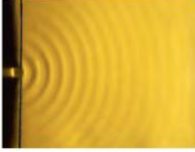
\includegraphics[scale = 1.5]{Ressources/TSPE_C9_Exercices_Fig2.png}
\end{multicols}

\section{Bulles de savon}
Lorsqu'un faisceau de lumière passe d'un milieu transparent, homogène et isotrope à un autre, une partie du faisceau est réfléchie, l'autre est réfractée. Les angles sont liés aux lois de Snell-Descartes.\\
Localement, une bulle de savon est modélisée comme une fine couche d'un matériau transparent entourée de deux autres milieux transparents d'indices différents. La différence de chemin optique $\delta$ entre le  rayon 1 et le rayon 2 ne dépend que de l'épaisseur $e$, de l'indice de réfraction $n$, de l'angle de réfraction $\beta$ et de la longueur d'onde $\lambda$ du faisceau incident :
\begin{eqnarray}
    \delta = 2 n \cdot e \cdot \cos(\beta) + \dfrac{\lambda}{2} \nonumber
\end{eqnarray}
\begin{center}
    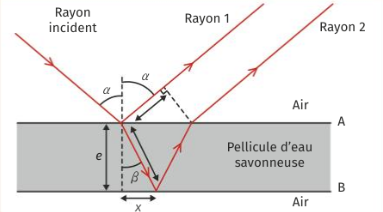
\includegraphics[scale = 1]{Ressources/TSPE_C9_Exercices_Fig3.png}
\end{center}

    \begin{enumerate}
    \item Exprimer la différence de chemin optique dans les cas d'interférence constructives et destructives.\\
    \textcolor{blue}{Pour que les interférences soient constructives, la différence de chemin optique doit respecter la relation $\delta = k\cdot \lambda$\\
    Pour des interférences destructives il faut que : $\delta = (k+ \frac{1}{2})\cdot \lambda$}
    \item On considère que l'observation se fait sous incidence normale ($\beta$ = 0 \unit{\radian}). Pour chacune des situations précédentes, établir l'expression de l'épaisseur $e$ du film d'eau savonneuse en fonction de $n$, $\lambda$ et $k$ (l'ordre d'interférences).\\
    \textcolor{blue}{Pour $\beta$ = 0, on aura la relation : $\delta = 2 n \cdot e \cdot \cos(0) + \dfrac{\lambda}{2}$, soit  : $\delta = 2 n \cdot e + \dfrac{\lambda}{2}$\\
    Pour des interférences constructives on aura : $\delta = 2 n \cdot e + \dfrac{\lambda}{2} =k\cdot \lambda$\\
    Soit : $e=\dfrac{\lambda(k-\dfrac{1}{2})}{2n}$\\
    Pour des interférences destructives on aura : $\delta = 2 n \cdot e + \dfrac{\lambda}{2} =(k+\frac{1}{2})\cdot \lambda$\\
    Soit : $e=\dfrac{\lambda\cdot k}{2n}$}
    \item Pour l'intervalle en longueur d'onde du domaine du visible [\num{400} \unit{\nano\meter} ; \num{800} \unit{\nano\meter}] et un indice de réfraction $n$ = \num{1,34}, calculer les épaisseurs $e$ du film dans les cas d'interférences constructives et destructives d'ordre 1 ($k$ = 1).\\
    \textcolor{blue}{Si on considère des interférences constructives d'ordre 1, dans les conditions de l'énoncé on aura :\\
    $e_{400nm}=\dfrac{\num{400e-9}\times (1-\dfrac{1}{2})}{2\times 1,34}$ = \num{7,46e-8} \unit{\meter}\\
    $e_{800nm}=\dfrac{\num{800e-9}\times (1-\dfrac{1}{2})}{2\times 1,34}$ = \num{1,49e-7} \unit{\meter}\\
    Dans le cas d'interférences constructives l'épaisseur $e$ serait dans l'intervalle [74,6 - 149 nm]\\    
    Si on considère des interférences destructives d'ordre 1, dans les conditions de l'énoncé on aura :\\
    $e_{400nm}=\dfrac{\num{400e-9}}{2\times 1,34}$ = \num{1,49e-7} \unit{\meter}\\
    $e_{800nm}=\dfrac{\num{800e-9}}{2\times 1,34}$ = \num{2,99e-7} \unit{\meter}\\
    Dans le cas d'interférences constructives l'épaisseur $e$ serait dans l'intervalle [149 - 299 nm]\\}
    
    \item Quand l'épaisseur $e$ du film devient supérieure à \num{30} \unit{\nano\meter}, plusieurs longueurs d'onde interfèrent. Pour une épaisseur de \num{900} \unit{\nano\meter}, déterminer les couples de valeurs $k$ et $\lambda$ pour lesquels des interférences constructives sont attendues. En déduire la couleur des franges.
    \end{enumerate}
\begin{multicols}{2}
\textcolor{blue}{Pour des interférences destructives on peut utiliser la relation précédente : $e=\dfrac{\lambda\cdot k}{2n}$, soit en isolant les termes recherchés : $\lambda=\dfrac{2e\cdot n}{k}$. \\ Avec les valeurs de l'énoncé on aura : $$\lambda = \dfrac{2 \times \num{900e-9} \times 1,34}{k} = \dfrac{\num{2,41e-6}}{k}$$
On aura dons les solutions suivantes :}
\begin{center}
  	\begin{tabular}{|c|c|}
    \hline k & $\lambda$ (en nm)\\
    \hline 1 & \num{2,41e3}\\
    \hline 2 & \num{1,21e3}\\
    \hline 3 & \num{804}\\
    \hline 4 & \num{60,3}\\
    \hline
    \end{tabular}
\end{center}
\columnbreak
\textcolor{blue}{Pour des interférences constructives, on peut utiliser la relation $e=\dfrac{\lambda(k-\dfrac{1}{2})}{2n}$. \\On peut déterminer les couples en transformant la formule pour donner :$\lambda=\dfrac{2e\cdot n}{k-\dfrac{1}{2}}$, soit $$\lambda=\dfrac{2\times \num{900e-9}\times 1,34}{k-\dfrac{1}{2}}$$
On aura donc les solutions suivantes :}
\begin{center}
\begin{tabular}{|c|c|}
    \hline k & $\lambda$ (en nm)\\
    \hline 1 & \num{4,82e3}\\
    \hline 2 & \num{1,61e3}\\
    \hline 3 & \num{964}\\
    \hline 4 & \num{689}\\
    \hline 5 & \num{53,6}\\
    \hline
    \end{tabular}
\end{center}
\end{multicols}
\textcolor{blue}{Les seules franges visibles seront celles provenant des interférences constructives, dans le domaine du visible, soit pour une longueur d'onde de 689 nm, correspondant à un rayonnement rouge.}

\begin{enumerate}
\setcounter{enumi}{5}
    \item Une zone blanche apparaît avant l'éclatement du film d'eau savonneuse. Expliquer pourquoi.\\
    \textcolor{blue}{Avant l'éclatement, l'angle d'observation de la bulle permet de voir une déclinaison de franges correspondant à la décomposition de la lumière blanche. Lorsque la bulle éclate elle se rétracte tout d'abord depuis le point d'éclatement jusqu'au point opposé. Cette rétractation va resserrer les franges observées vers un point. La superposition des longueur d'onde va donner de la lumière blanche.}
\end{enumerate}

\section{Interféromètre de Michelson}
\begin{multicols}{2}
De nos jours, l'interféromètre de Michelson peut être utilisé pour mesurer avec précision la longueur d'onde d'une source lumineuse monochromatique.\\
Un faisceau de lumière issu d'une source laser est séparé en deux au point $A$ d'une lame séparatrice semi-réfléchissante. Chacun des deux faisceaux ainsi formés est alors en phase. Ils constituent un système de deux sources cohérentes.\\
Ces deux faisceaux sont réfléchis par des miroirs plans $M_1$ et $M_2$ (respectivement aux points $B$ et $C$) et redirigés vers le point $A$ de la lame séparatrice pour finalement se rejoindre au niveau d'un capteur qui mesure l'intensité lumineuse résultante.\\
L'un des miroirs (le miroir $M_1$ par exemple) est placé sur un chariot motorisé afin de le faire glisser lentement et de façon continu. Le mouvement du chariot modifie le trajet de l'un des faisceaux, modifiant l'intensité lumineuse mesurée par le capteur : on observe une alternance d'interférences constructives et destructives.
\begin{center}
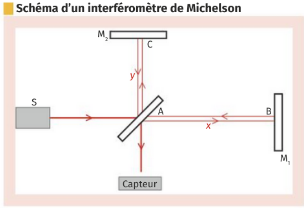
\includegraphics{Ressources/TSPE_C9_Exercices_Fig5.png}
\end{center}
\end{multicols}
\begin{enumerate}
    \item Exprimer la différence de chemin optique $\delta$ entre les deux faisceaux en fonction des distances $x$ et $y$.\\
    \textcolor{blue}{Les faisceaux se séparent au point $A$ :
    \begin{itemize}
        \item une première partie du faisceau parcourt deux fois la distance AB (soit $2x$) avant de parcourir la distance entre A et le capteur.
        \item un deux deuxième partie du faisceau parcourt deux fois la distance AC (soit $2y$) avant de parcourir la distance entre A et le capteur.
    \end{itemize}
    On peut exprimer $\delta$ comme étant $\delta = 2x - 2y = 2(x-y)$.}
    \item Lorsque $x=y$, préciser ce qu'enregistre le capteur.\\
    \textcolor{blue}{Lorsque $x = y$, les deux signaux lumineux sont en phase, le capteur pourra donc capteur une interférence constructive.}
\end{enumerate}
Quand le chariot démarre et s'arrête, le capteur enregistre une intensité maximale. Pendant le déplacement d'une distance $d$ du miroir $M_1$ le capteur a enregistré une alternance de 6522 plages sombres.
\begin{enumerate}
\setcounter{enumi}{2}
    \item Donner l'expression de la différence de chemin optique $\delta$ en fonction de $d$.\\
    \textcolor{blue}{Sur le déplacement $d$, le capteur a enregistré 6522 plages sombres, soit autant d'interférences destructives. La différence de chemin optique est donc de $\delta = 2(x-y) = 2d$}
    \item Donner l'expression de la différence de chemin optique $\delta$ en fonction de la longueur d'onde dans le cas d'interférences constructives.\\
    \textcolor{blue}{Dans le cas d'interférences constructives, on aura $\delta = k\cdot \lambda$, avec $k$ l'ordre d'interférence, c'est à dire le nombre d'interférences constructives rencontrées.}
    \item En déduire la longueur d'onde $\lambda$ du laser pour un déplacement $d$ = \num{2,064} \unit{\milli\meter} du miroir.
    \textcolor{blue}{Pour $d$ = 2,064 \unit{\milli\meter} et $k$ = 6522, on aura :  $\lambda = \dfrac{2 \times\num{ 2,064e-3}}{6522}$ = \num{6,33e-7} \unit{\meter}.\\
    Il s'agit d'un laser de longueur d'onde $\lambda$ = 633 \unit{\nano\meter}.}
\end{enumerate}

\end{document}